\chapter{Arhitectura Hardware}
\thispagestyle{pagestyle}
\section{Schema hardware bloc a sistemului}

\begin{figure}[h]
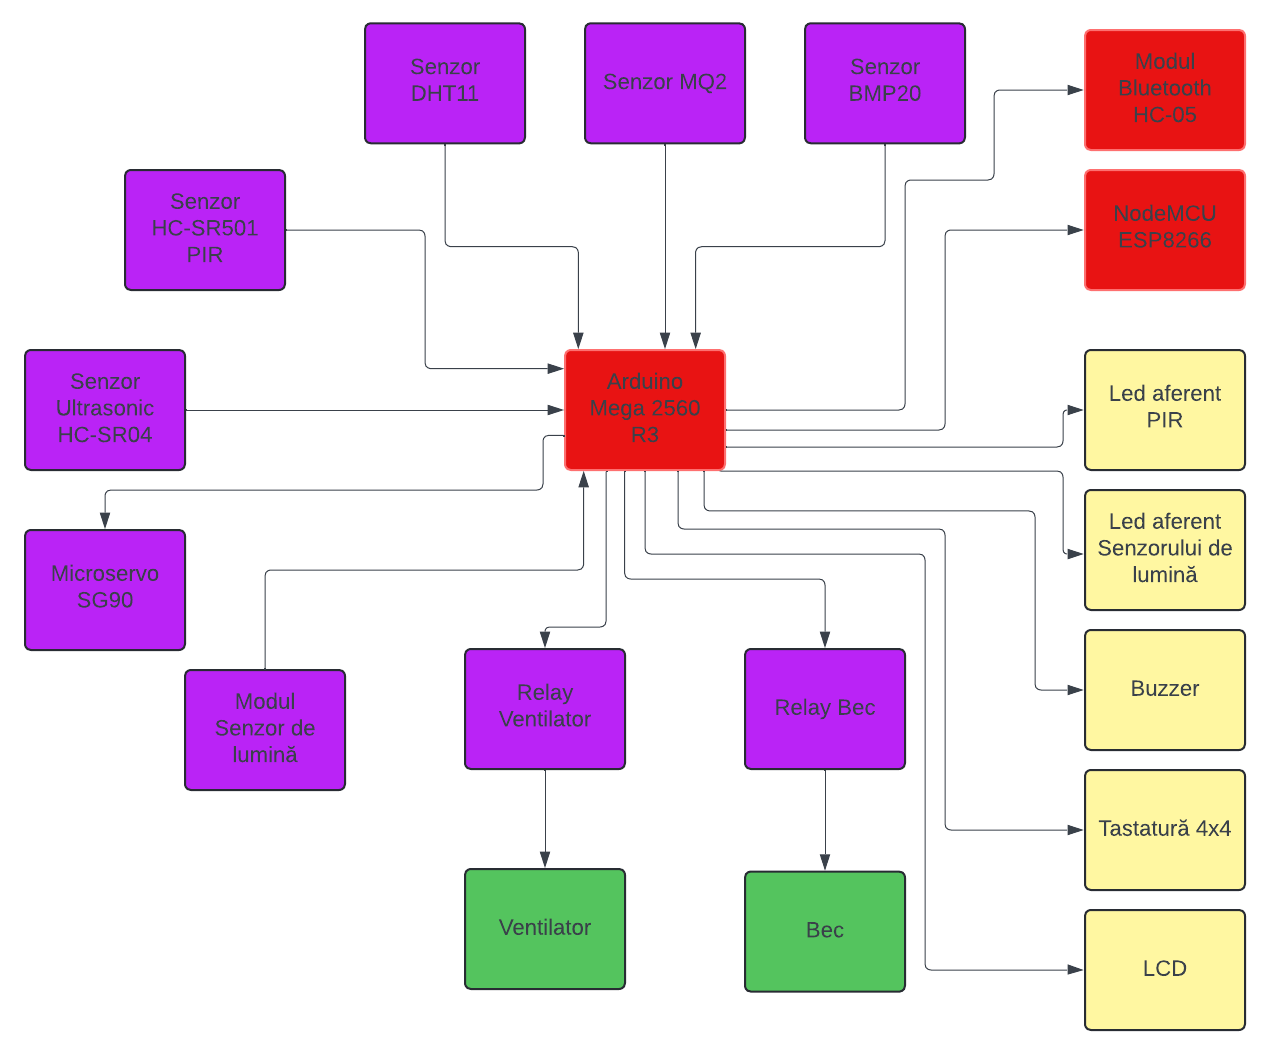
\includegraphics[width=1\textwidth]{bachelors_ro/images/schema_bloc.png}
\caption{Schema hardware bloc a sistemului}
\label{fig:schema_bloc}
\end{figure}

În figura \ref{fig:schema_bloc} este prezentată schema bloc a sistemului modelat de mine. Scopul acestei arhitecturi este de a controla componente precum led-urile, servomotorul și buzzer-ul cu ajutorul datelor oferite de senzori. Astfel, componentele din chenarele mov reprezintă componentele ce oferă diverse date (senzori), iar cel verzi și galbene reprezintă componentele ce execută diverse funcții conform necesităților aferente. În chenarele roșii sunt componentele ce primesc informații interpretate de placa de dezvoltare Arduino Mega și le trimit mai departe prin intermediul WiFi-ului către Cloud-ul Blynk și prin Bluetooth către aplicația Andorid.

Majoritatea senzorilor sunt legați folosind fire la pinii digitali ai plăcii, cu excepția senzorului MQ2 ce este conectat la un pin analogic și senzor BMP280 ce folosește protocolul I2C. Legătura dintre Arduino Mega cu Modulul Bluetooth, respectiv NodeMCU ESP8266, se face prin interfețele seriale UART oferite de placă.

\section{Realizarea montajului arhitecturii Hardware}
Pentru a realiza montajul afarent arhitecutrii implementate am ales să folosesc o placă dedicată PCB (Printed Circuit Board). Astfel, am lipit direct pe aceasta placa de dezvoltare Arduino Mega, NodeMCU ESP8266 și modul de Bluetooth HC-05 cu ajutorul cositorului și a gărdulețelor de pini. Pentru modulul Bluetooth și NodeMCU am folosit jumpere pentru a putea întrerupe comunicarea serială între acestea și Arduino Mega, deoarce aceasta trebuie să fie oprită dacă doresc să urc cod nou pe placa Arduino Mega, dar și pe NodeMCU. 

Pentru restul componentelor am folosit fire de diverse culori și grosimi pentru a fi mai ușor identificabile. Aceste cabluri au lipite direct de pinii plăcii Arduino cu cositor, iar la capete au fost modificate fie cu mufe mama, fie cu mufe tată în funcție de nevoie. În Figura \ref{fig:sechema_full_sistem} este prezentată schema de conectare a întregului sistem.

\begin{figure}[H]
    \centering
    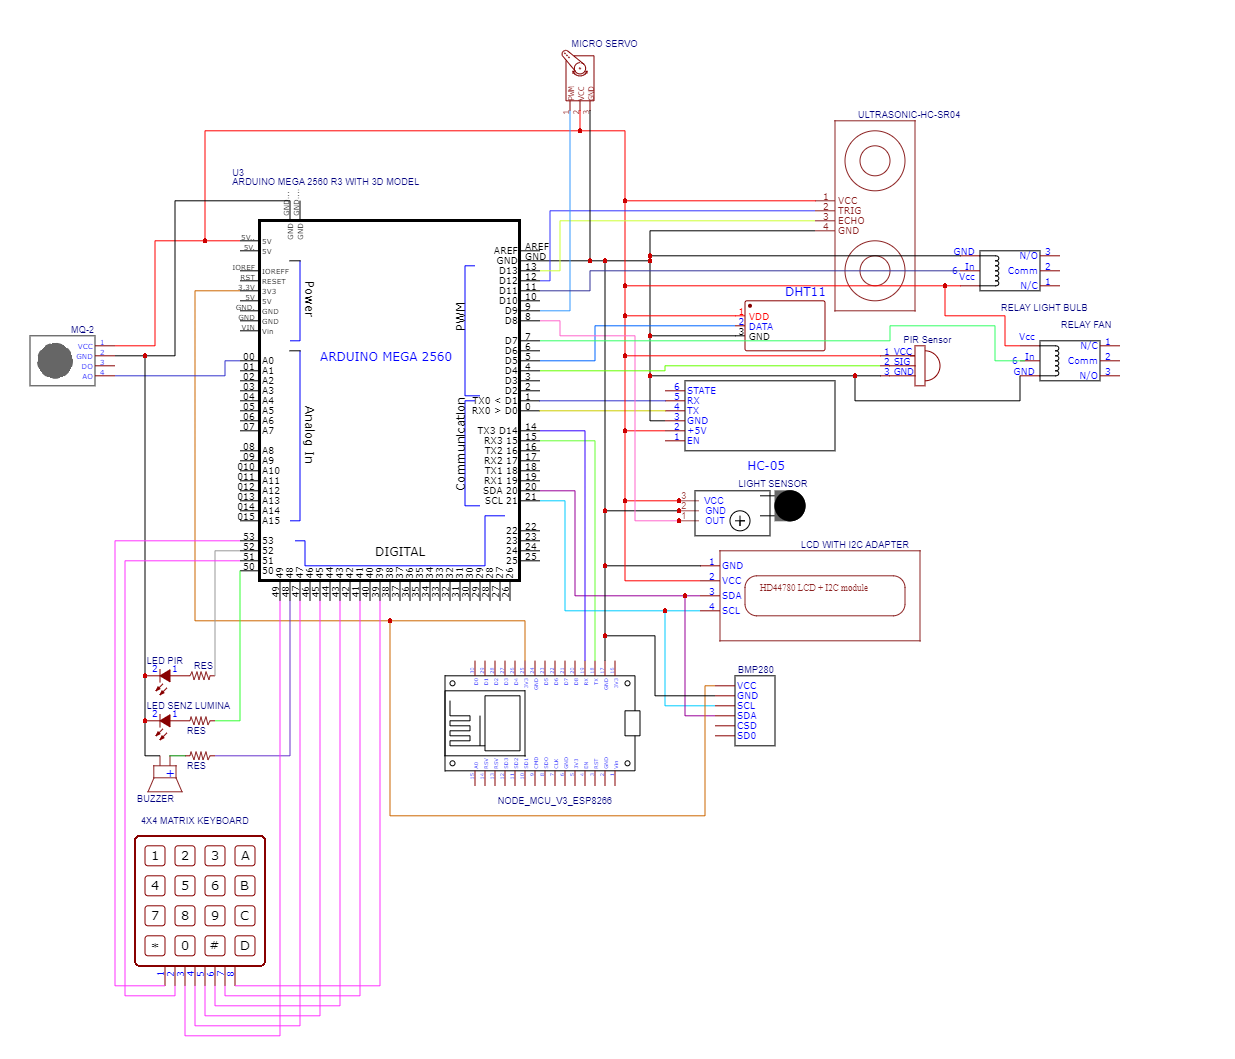
\includegraphics[width=1\linewidth]{bachelors_ro/images/sechema_full_sistem.png}
    \caption{Schema de conectare a sistemuui}
    \label{fig:sechema_full_sistem}
\end{figure}